\newif\ifshowsolutions
\showsolutionsfalse
\documentclass{article}
\usepackage{listings}
\usepackage{amsmath}
\usepackage{subfig}
\usepackage{amsthm}
\usepackage{amsmath}
\usepackage{amssymb}
\usepackage{graphicx}
\usepackage{mdwlist}
\usepackage{geometry}
\usepackage{titlesec}
\usepackage{palatino}
\usepackage{mathpazo}
\usepackage{fancyhdr}
\usepackage{paralist}
\usepackage{todonotes}
\usepackage{tikz}
\usepackage{float} % Place figures where you ACTUALLY want it
\usepackage{comment} % A hack to toggle sections
\usepackage{ifthen}
\usepackage{mdframed}
\usepackage{verbatim}
\usepackage{listings}
\usepackage{bbm}
\usepackage{upquote} % Prevents backticks replacing single-quotes in verbatim
\usepackage{listings}
\lstset{basicstyle=\ttfamily,
  showstringspaces=false,
  commentstyle=\color{red},
  keywordstyle=\color{blue}
}
\usepackage[strings]{underscore}
\usepackage[colorlinks=true]{hyperref}
\usetikzlibrary{positioning,shapes,backgrounds}

\geometry{margin=1in}
\geometry{headheight=2in}
\geometry{top=2in}

\setlength{\marginparwidth}{2.15cm}
\setlength{\parindent}{0em}
\setlength{\parskip}{0.6\baselineskip}

\rhead{}
\lhead{}

% Spacing settings.
\titlespacing\section{0pt}{12pt plus 2pt minus 2pt}{0pt plus 2pt minus 2pt}
\titlespacing\subsection{0pt}{12pt plus 4pt minus 2pt}{0pt plus 2pt minus 2pt}
\titlespacing\subsubsection{0pt}{12pt plus 4pt minus 2pt}{0pt plus 2pt minus 2pt}
\renewcommand{\baselinestretch}{1.15}

% Shortcuts for commonly used operators.
\newcommand{\E}{\mathbb{E}}
\newcommand{\Var}{\operatorname{Var}}
\newcommand{\Cov}{\operatorname{Cov}}
\newcommand{\Bias}{\operatorname{Bias}}
\DeclareMathOperator{\argmin}{arg\,min}
\DeclareMathOperator{\argmax}{arg\,max}

% Do not number subsections and below.
\setcounter{secnumdepth}{1}

% Custom format subsection.
\titleformat*{\subsection}{\large\bfseries}

% Set up the problem environment.
\newcounter{problem}[section]
\newenvironment{problem}[1][]
{\begingroup
  \setlength{\parskip}{0em}
  \refstepcounter{problem}\par\addvspace{1em}\textbf{Problem~\Alph{problem}\!
    \ifthenelse{\equal{#1}{}}{}{ [#1 points]}:}
  \endgroup}

% Set up the subproblem environment.
\newcounter{subproblem}[problem]
\newenvironment{subproblem}[1][]
{\begingroup
  \setlength{\parskip}{0em}
  \refstepcounter{subproblem}\par\medskip\textbf{\roman{subproblem}.\!
    \ifthenelse{\equal{#1}{}}{}{ [#1 points]:}}
  \endgroup}

% Set up the teachers and materials commands.
\newcommand\teachers[1]
{\begingroup
  \setlength{\parskip}{0em}
  \vspace{0.3em} \textit{\hspace*{2em} TAs responsible: #1} \par
  \endgroup}
\newcommand\materials[1]
{\begingroup
  \setlength{\parskip}{0em}
  \textit{\hspace*{2em} Relevant materials: #1} \par \vspace{1em}
  \endgroup}

% Set up the hint environment.
\newenvironment{hint}[1][]
{\begin{em}\textbf{Hint: }}
    {\end{em}}


% Set up the solution environment.
\ifshowsolutions
  \newenvironment{solution}[1][]
  {\par\medskip \begin{mdframed}\textbf{Solution~\Alph{problem}#1:} \begin{em}}
        {\end{em}\medskip\end{mdframed}\medskip}
  \newenvironment{subsolution}[1][]
  {\par\medskip \begin{mdframed}\textbf{Solution~\Alph{problem}#1.\roman{subproblem}:} \begin{em}}
        {\end{em}\medskip\end{mdframed}\medskip}
\else
  \excludecomment{solution}
  \excludecomment{subsolution}
\fi

\usepackage[style=phys,
biblabel=brackets,
]{biblatex}
\DeclareSourcemap{
 \maps[datatype=bibtex,overwrite=true]{
  \map{
    \step[fieldsource=Collaboration, final=true]
    \step[fieldset=usera, origfieldval, final=true]
  }
 }
}
\renewbibmacro*{author}{
  \iffieldundef{usera}{
    \printnames{author}
  }{
    \printfield{usera} Collaboration
  }
}
\addbibresource{final_projects.bib}

\chead{
  {\vbox{
      \vspace{2mm}
      \large
      Computational Physics II \hfill
      UCSD PHYS 142/242 \hfill \\[1pt]
      Final Projects\hfill
      Presentations: Monday, March 10 - Friday, March 14, 2025\\
	  \hfill
	  Report and code due: Friday, March 21, 2025, 8:00pm\\
    }
  }
}


\begin{document}
\pagestyle{fancy}

\section*{Instructions}
\begin{itemize}
  \item You will be assigned to a group of 3--4 students and part of the project is to learn how to collaborate effectively.
        So, meet with your group members to discuss the project and divide the work.
  \item The project will be graded based on the quality of the report and code, the correctness of the results, and the depth of the analysis.
  \item The projects outlined here are designed to be open-ended, and give you the freedom to explore additional topics that we may not have covered in class.
  \item The presentation should be about 20 minutes and different group members should deliver different parts of it.
  \item The presentation/report should include an introduction to the problem, a description of the methods used (and why), and a discussion of the results.
  \item You should submit all code as a public GitHub repository with a README that explains how to run it.
        You are also encouraged to use GitHub to collaborate with your group members.
  \item The report should be about 4 pages, including figures and tables, but excluding references.
        It should be double column using the \emph{Phys. Rev. Lett.} template.
  \item Please submit your report as a single .pdf file to Gradescope under ``Final Project Report".
        The report should include a link to your public GitHub repository.        The .zip file should contain all of your source code files.
  \item Fill out your project preferences here: \url{https://forms.gle/exB5BEtVddbvmGDr7}
\end{itemize}

\newpage
\section{Double Well Potential with MCMC}

Consider the double well potential,
\begin{equation}
  V(x) =  \alpha x^4  - 2x^2 + \frac{1}{\alpha}
\end{equation}
where $x$ is the position of the particle, and we set $m=\hbar=1$ and $\alpha = 0.4$.
See Refs.~\cite{Mittal:2020,Rodgers:2014} for discussions of similar problems.

Use the path integral formulation with imaginary time $\tau$,
\begin{align}
  Z & = \int \mathcal D x(\tau) \exp\left [-\frac{1}{\hbar}\oint^{\tau_b}_{0} L_E(x(\tau)) d\tau \right]]                                                                                                                                                                                        \\
    & =\lim_{\delta\tau\to 0}   \int \cdots \int dx_0\cdots dx_{N-1}  \left (\frac{2\pi \hbar \delta\tau}{m} \right)^{-\frac{N}{2}} \exp\left [-\frac{1}{\hbar} \left(\sum_{i=1}^{N}\frac{m(x_{i} - x_{i-1})^2}{2\delta\tau} + \delta\tau V \left(\frac{x_{i-1}+x_{i}}{2}\right )\right)\right ]
\end{align}
where $L_E(x(\tau)) = \textstyle\frac{m}{2} \left(\frac{dx}{d\tau}\right)^2 + V(x(\tau))$ is the Euclidean Lagrangian, imaginary time is discretized with $N$ increments, $\tau_a = 0$, and $\tau_b = N\delta\tau = \hbar\beta$.
So the probability of a given path $(x_0, x_1, \dots, x_{N-1})$ is
\begin{align}
  p(x_0,\dots, x_{N-1}) & \propto \exp\left [-\frac{1}{\hbar} \left(\sum_{i=1}^{N}\frac{m(x_{i} - x_{i-1})^2}{2\delta\tau} + \delta\tau V \left(\frac{x_{i-1}+x_{i}}{2}\right )\right)\right ]
\end{align}

\begin{problem}
Evaluate the ground state energy and probability distribution of the particle using Markov chain Monte Carlo with the Metropolis-Hastings algorithm in the large-$\tau_b$ (imaginary time) limit.
Describe your strategy for determining $\tau_b$, the initial configuration, burn-in steps, hit size, number of sweeps, and thinning (if any).
\end{problem}

\begin{problem}
Plot the ground state probability distribution and compare it with the expected form.
\end{problem}

\begin{problem}
Calculate the energy and probability distribution of the particle from the same simulation code for a smaller value of $\tau_b$.
What is the expected probability distribution in this case?
What does this correspond to in terms of a statistical mechanics interpretation?
\end{problem}


\newpage
\section{2D Ising Model with MCMC}

Consider the 2D Ising model in a square lattice $\Lambda$ with $100\times 100$ sites and periodic boundary conditions in the presence of an external magnetic field $B$.
The energy of the system for a given spin configuration $\sigma = \{\sigma_i\}_{i\in \Lambda}$ is
\begin{equation}
  E(\sigma) = -J\sum_{\langle ij\rangle} \sigma_i\sigma_j - B\sum_{i\in \Lambda} \sigma_i,
\end{equation}
where $\langle i j \rangle$ denotes two adjacent sites (with no double counting), $J$ is the spin-spin interaction, and $\sigma_i \in \{ -1, +1\}$ is the spin at site $i$.

The magnetization of the system is
\begin{equation}
  M(\sigma) = \frac{1}{|\Lambda|}\sum_{i\in \Lambda} \sigma_i.
\end{equation}

\begin{problem}
Use Markov chain Monte Carlo and the Metropolis-Hastings algorithm to simulate the 2D Ising model at different temperatures $T$ and magnetic field strengths $B$.
Discuss your strategy for determining the initial configuration, burn-in steps, total number of steps, and thinning (if any).
\end{problem}


\begin{problem}
Plot 1D scans of the magnetization $M$ versus $T$ for fixed $B$ at three different values: $B<0$, $B=0$, and $B>0$.
Plot 1D scans of the magnetization $M$ versus $B$ for fixed $T$ at three different values: $T<T_C$, $T=T_C$, and $T>T_C$, where $T_C=\frac{2}{\ln(1+\sqrt{2})}\approx 2.269$.
\end{problem}

\begin{problem}
Putting this all together, draw/describe the phase diagram in $B$ versus $T$ of the 2D Ising model, where the magnetization $M$ is the order parameter.
Consider discussing first-order phase transitions and critical exponents, hysteresis and metastable states, and/or specific heat and susceptibility.
See Refs.~\cite{Eastman:2014,Krauss:2018} for relevant discussions.
\end{problem}

\newpage
\section{Drell--Yan Event Generator with VEGAS}

Consider the Drell--Yan production process at an electron-positron collider, in which an electron and positron collide to produce a virtual photon or a $Z$ boson that then decays into a muon-antimuon pair, $e^+e^-\to Z/\gamma \to \mu^+\mu^-$.

\begin{center}
  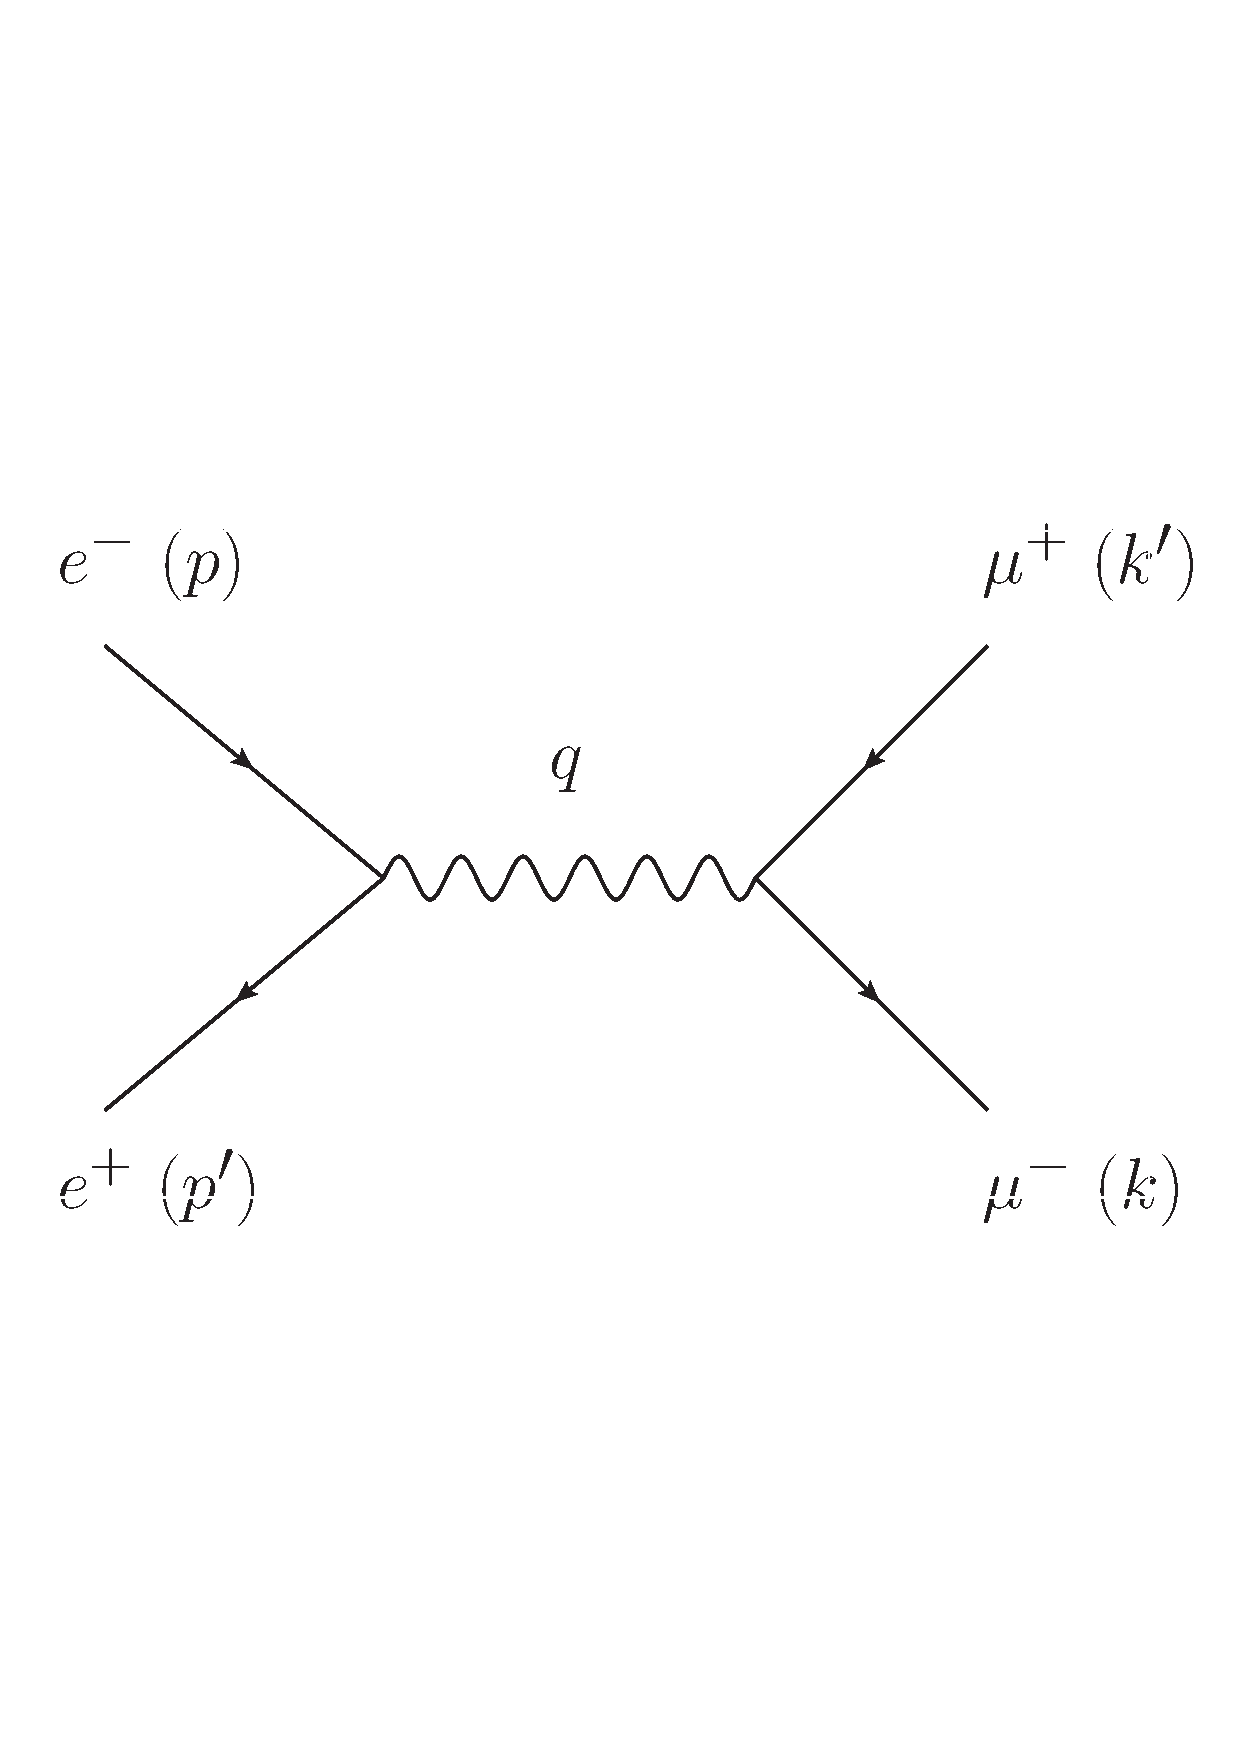
\includegraphics[width=0.45\textwidth]{eemumu.pdf}
  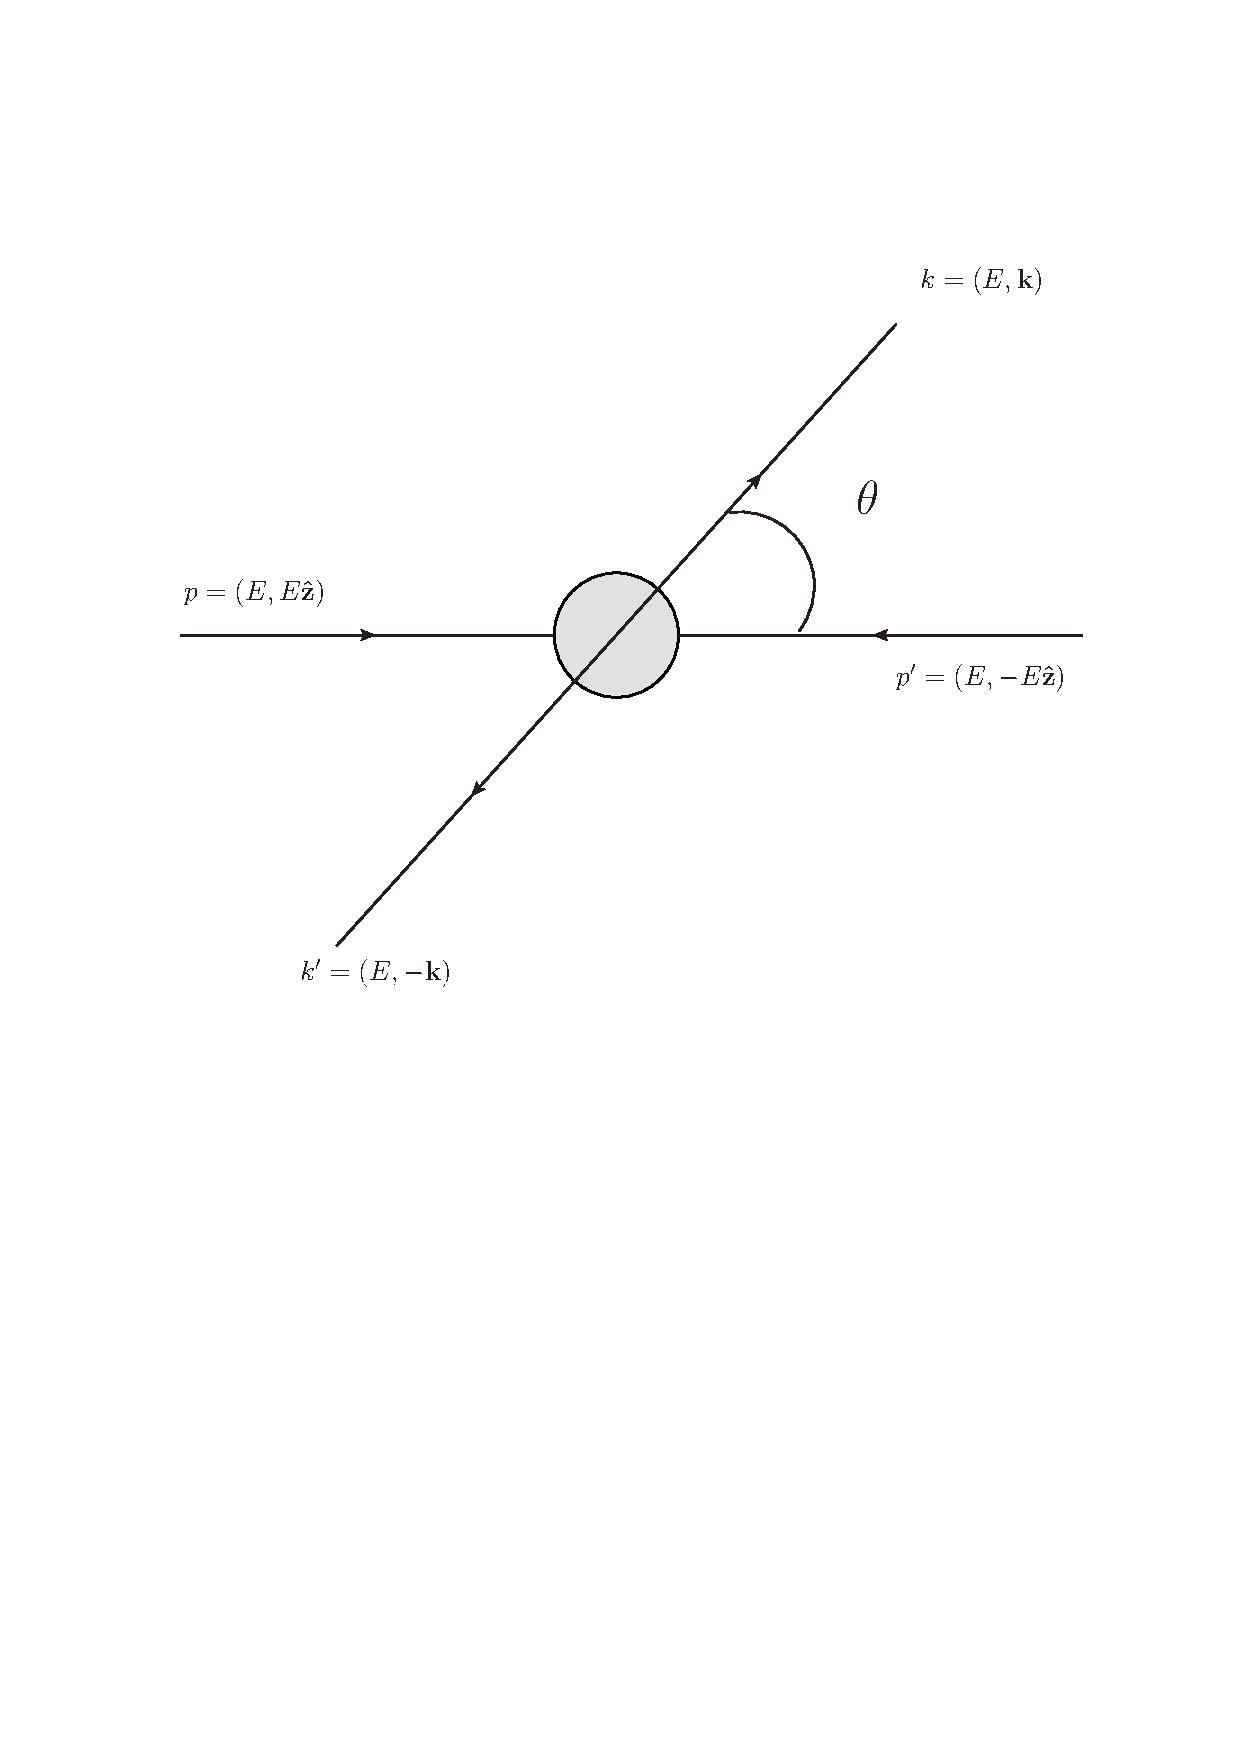
\includegraphics[width=0.45\textwidth]{eemumukin.pdf}
\end{center}

As described in lecture and in Ref.~\cite{Papaefstathiou:2014mya}, the differential cross section for center-of-mass energy $E_\text{CM} = \sqrt{\hat s}$ and scattering angle $\theta$ is given by
\begin{equation}
  \label{eq:partonicxs}
  \frac{ d\sigma } { d \Omega }(\hat s, \cos\theta) = \frac{\alpha^2}{4 \hat{s} } \left[ A_0 (\hat s) ( 1  + \cos ^2 \theta ) + A_1(\hat s) \cos \theta \right] \;,
\end{equation}
where $A_0$ and $A_1$ are given by
\begin{align}
  A_0(\hat s) & = Q_e^2 - 2 Q_e V_\mu  V_e ~\chi_1(\hat s) + (A_\mu^2 + V_\mu^2)  (A_e^2 + V_e^2)  ~\chi_2(\hat s)\;, \nonumber \\
  A_1(\hat s) & = -4 Q_e  A_\mu A_e ~\chi_1(\hat s) + 8 A_\mu V_\mu A_e V_e ~ \chi_2(\hat s)\;,
\end{align}
and the $\chi_1$ and $\chi_2$ are given by
\begin{align}
  \chi_1 (\hat{s}) & = \kappa \hat{s} ( \hat{s} - M_Z^2 ) / (  (\hat{s}-M_Z^2)^2 + \Gamma_Z^2 M_Z^2 ) \;, \nonumber \\
  \chi_2 (\hat{s}) & = \kappa^2 \hat{s}^2 / (  (\hat{s}-M_Z^2)^2 + \Gamma_Z^2 M_Z^2 ) \;, \nonumber                 \\
  \kappa           & = \sqrt{2} G_F M_Z^2 / (4 \pi \alpha) \;.
\end{align}

Useful constants are given in the tables below.

\begin{center}
  \begin{tabular}{llll}
    Fermions                       & $Q_f$          & $V_f$                                            & $A_f$          \\ \hline
    $u$, $c$, $t$                  & $+\frac{2}{3}$ & $(+\frac{1}{2} - \frac{4}{3} \sin ^2 \theta_W )$ & $+\frac{1}{2}$ \\
    $d$, $s$, $b$                  & $-\frac{1}{3}$ & $(-\frac{1}{2} - \frac{2}{3} \sin ^2 \theta_W )$ & $-\frac{1}{2}$ \\
    $\nu_e$, $\nu_\mu$, $\nu_\tau$ & $0$            & $\frac{1}{2}$                                    & $+\frac{1}{2}$ \\
    $e$, $\mu$, $\tau$             & $-1$           & $(-\frac{1}{2} + 2 \sin ^2 \theta_W )$           & $-\frac{1}{2}$ \\
  \end{tabular}
\end{center}

\begin{center}
  \begin{tabular}{lll}
    Variable             & Symbol                        & Value                                  \\ \hline
    conversion factor    & GeV$^{-2}\leftrightarrow$\,pb & $3.894\times 10^8$\,pb = 1\,GeV$^{-2}$ \\
    $Z$ boson mass       & $M_Z$                         & 91.188\,GeV                            \\
    $Z$ boson width      & $\Gamma_Z$                    & 2.4414\,GeV                            \\
    QED running coupling & $\alpha$                      & $\frac{1}{132.507}$                    \\
    Fermi constant       & $G_F$                         & $1.16639\times 10^{-5}$~GeV$^{-2}$.    \\
    Weinberg angle       & $\sin^2 \theta_W$             & 0.222246                               \\
  \end{tabular}
\end{center}

\begin{problem}
Use standard acceptance-rejection Monte Carlo to generate events $(E_\text{CM}, \cos\theta)$ for the Drell--Yan process in a range $E_\text{CM} \in [10, 200]\,\text{GeV}$ and $\cos\theta \in [-1, 1]$.
Note, usually $E_\text{CM}$ is fixed in an electron-positron collider, but we will consider a range of energies, which is similar to the situation at a hadron collider where the partonic center-of-mass energy is not known exactly.
\end{problem}

\begin{problem}
Use the VEGAS Monte Carlo method~\cite{Lepage:1977sw,Lepage:2020tgj} to generate events $(E_\text{CM}, \cos\theta)$ for the Drell--Yan process in a range $E_\text{CM} \in [10, 200]\,\text{GeV}$ and $\cos\theta \in [-1, 1]$.
Compare how many function evaluations are needed to arrive at the same number of samples, e.g. 10,000.
Discuss the settings you use for the VEGAS algorithm, i.e. how many iterations, what kind of damping factor, and how many bins, etc.
\end{problem}

\newpage

\noindent\textbf{\emph{Bibliography}}:\\
\printbibliography[heading=none]

\end{document}
